\documentclass[12pt,a4paper]{article}
\usepackage[utf8]{inputenc}
\usepackage[T1]{fontenc}
\usepackage[english]{babel}
\usepackage{lmodern}
\usepackage{microtype}
\usepackage{amsmath, amssymb, amsfonts}
\usepackage[margin=2.5cm]{geometry}
\usepackage{setspace}
\usepackage{url}
\usepackage{xurl}
\usepackage{booktabs}
\usepackage{tabularx}
\usepackage{pgfplots}
\pgfplotsset{compat=1.18}
\usetikzlibrary{babel}

\onehalfspacing

\title{\textbf{Stationary Strings XII: Dark-Matter-Free Galactic Dynamics, the Meral Cosmic Acceleration Scale, SPARC Rotation Curves, and EHT Black-Hole Ring Evidence} \\[0.3cm]
\large (Baryonic Tully--Fisher Relation and Sgr A*/M87* Ring Saturation, No New Calibration Constant)}
\author{Fahri Meral}
\date{October 19, 2026}

\begin{document}

\maketitle

\begin{abstract}
As the application of the locked constants of the Stationary
Strings Theorem I--X series
($\Lambda_{\mathrm{Meral}}^{(0)} = 0.07226943267767906$,
$\mu_s^{\mathrm{Meral}} = 2\sqrt{2}\,\Lambda_{\mathrm{Meral}}^{(0)} = 0.2044088237$,
$\beta_0 = 1/2$, $\eta_{\mathcal{T}_0} = 0.1434$,
$\mathcal{C}_{\mathrm{univ}} = 1.626038$) to galactic and cosmological scales,
this study establishes halo-free galaxy dynamics with no dark matter:
\begin{enumerate}
    \item \textbf{Meral Cosmic Acceleration Scale (Theorem XII.1, Test T29):}
    From Planck 2018 $H_0$,
    $a_{\mathrm{Meral}} = \mu_s^{\mathrm{Meral}}(1-\eta_{\mathcal{T}_0})\,cH_0
    = 1.146589\times 10^{-10}\,\mathrm{m/s}^2$, agreeing with the
    153-galaxy SPARC measurement
    $a_0^{\mathrm{SPARC}} = (1.20\pm 0.02\pm 0.24)\times
    10^{-10}\,\mathrm{m/s}^2$ to 4.45\% ($0.22\,\sigma_{\mathrm{sys}}$).
    \item \textbf{RAR and Baryonic Tully--Fisher (Theorem XII.2, Tests T29--T30):}
    The string-loop tension gives
    $g_{\mathrm{obs}} = g_{\mathrm{bar}}[1+(x+x^2)^{-1/2}]$
    ($x = g_{\mathrm{bar}}/a_{\mathrm{Meral}}$); in the outer-halo limit
    $v_{\mathrm{flat}}^4 = GM_b a_{\mathrm{Meral}}$ with log-log slope exactly
    $4.0$ ($|m-4|<10^{-14}$, $R^2 = 1.0$). Across five SPARC archetypes the mean
    absolute relative error is 4.54\%, four of them below 4.1\%
    (giant spiral UGC 2885 is an openly reported 12.9\% outlier).
    \item \textbf{EHT Black-Hole Ring Saturation (Theorem XII.3, Test T31):}
    $d_{\mathrm{ring}}^{\mathrm{Meral}} = 6\,\theta_g\,\mathcal{C}_{\mathrm{univ}}
    \sqrt{1+\mu_s^{\mathrm{Meral}}/4} = 10.002404\,\theta_g$ predicts
    $50.31\,\mu\mathrm{as}$ for Sgr A* ($0.65\,\sigma$) and
    $38.31\,\mu\mathrm{as}$ for M87* ($1.23\,\sigma$); the fractional ring width
    $\mu_s^{\mathrm{Meral}} = 0.2044 < 0.25$ satisfies the EHT bound.
\end{enumerate}
The numerical verification chain \texttt{T1--T31 (31/31 PASS)} and the
independent cross-check script (\path{mini_check_gp1.py}, \texttt{15/15 PASS})
fully pass.
\end{abstract}

\section{Introduction and Scientific Honesty Framework \\ (Exact Theorem vs.\ Observation vs.\ Cosmological Bridge Model)}

Flat outer rotation curves ($v(r)\to v_{\mathrm{flat}}$) and the Baryonic
Tully--Fisher relation ($v_{\mathrm{flat}}^4 = GM_b a_0$) have for ninety years
been explained either by hypothetical dark-matter halos or by Milgrom's (1983)
empirical acceleration constant [1--4]. The FENE-P cylindrical flux-string loop
tension and rational curvature factor locked through Stationary Strings
Theorems V--X [5--9], applied to vacuum flux-strings stretched across the
de Broglie/Hubble horizon, add a dark-matter-free elastic loop acceleration to
the centripetal equation.

\textbf{Three-layer honesty separation:}
\begin{itemize}
    \item \textbf{Exact Mathematical Theorem:} the $a_{\mathrm{Meral}}$
    definition (Eq.~\ref{eq:ameral}), the RAR interpolation (Eq.~\ref{eq:rar}),
    $v_{\mathrm{flat}}^4 = GM_b a_{\mathrm{Meral}}$, and the ring diameter
    (Eq.~\ref{eq:ring}) --- with no new calibration constant.
    \item \textbf{Observational literature (outside the model):} Planck 2018
    $H_0$ [8], McGaugh--Lelli--Schombert SPARC RAR/BTFR data [2,3], and
    EHT M87* [9] and Sgr A* [10] ring diameters.
    \item \textbf{Cosmological bridge model (open to test):} horizon-scale
    strings transmitting acceleration to the galactic plane, the exponential-disk
    baryon distribution, and the ring-width $\sim \mu_s$ ansatz.
\end{itemize}
Locked inputs: $\Lambda_{\mathrm{Meral}}^{(0)} = 0.07226943267767906$,
$\mu_s^{\mathrm{Meral}} = 0.2044088237$, $\beta_0 = 1/2$,
$\eta_{\mathcal{T}_0} = 0.1434$,
$\mathcal{C}_{\mathrm{univ}} = 1.626038$. No new calibration parameters.

\section{Task 23 / Test T29 --- Meral Scale and BTFR}

With Planck 2018 [8] $H_0 = 67.4\pm 0.5\,\mathrm{km\,s^{-1}\,Mpc^{-1}}$ the
cosmic horizon acceleration is
$a_H = cH_0 = 6.548322\times 10^{-10}\,\mathrm{m/s}^2$. Under the Theorems V--IX
coupling $\mu_s^{\mathrm{Meral}}$ and tangential suppression
$(1-\eta_{\mathcal{T}_0}) = 0.8566$, the effective string-loop acceleration is:

\textbf{Theorem XII.1 (Meral Cosmic Acceleration Scale):} \textit{The
elastic loop acceleration transmitted from the horizon to the
galactic plane:}
\begin{equation}
\label{eq:ameral}
\boxed{a_{\mathrm{Meral}} = \mu_s^{\mathrm{Meral}}\,(1-\eta_{\mathcal{T}_0})\,cH_0
= 2\sqrt{2}\,\Lambda_{\mathrm{Meral}}^{(0)}\,(1-\eta_{\mathcal{T}_0})\,cH_0.}
\end{equation}
The dimensionless factor
$\kappa_{\mathrm{Meral}} = 0.2044088237\times 0.8566 = 0.1750965984$
(comparable to $1/2\pi = 0.159155$) gives
\begin{equation}
a_{\mathrm{Meral}} = 0.1750965984\times 6.548322\times 10^{-10}
= \mathbf{1.146589\times 10^{-10}}\,\mathrm{m/s}^2.
\end{equation}
The axial $\sqrt{3}/2$ projection is $1.159205\times 10^{-10}$ and the local
$H_0 = 70.5$ value is $1.199325\times 10^{-10}\,\mathrm{m/s}^2$.
The observed $a_0^{\mathrm{SPARC}} = (1.20\pm 0.02\pm 0.24)\times 10^{-10}$ [2]
agrees to 4.45\% ($0.22\,\sigma_{\mathrm{sys}}$).

\textbf{Honesty caveat (audit record):} $a_{\mathrm{Meral}}$ is directly
proportional to $H_0$, so its comparison with $a_0$ depends largely on the
choice of $H_0$. The model predicts a \emph{dimensionless ratio}, not an
absolute acceleration scale:
$$\kappa_{\mathrm{Meral}}=\frac{a_{\mathrm{Meral}}}{cH_0}
=\frac{a_0}{cH_0}=0.175097 .$$
This ratio differs from the observed $a_0$ by 4.45\% with Planck 2018
($H_0=67.4$) and by 0.06\% with the local $H_0=70.5$; the test therefore
probes the ratio together with the adopted $H_0$, not an $H_0$-independent
absolute scale. The T29 agreement therefore shows consistency, not
validation, of the ratio $\mu_s^{\mathrm{Meral}}(1-\eta_{\mathcal{T}_0})$.

Radial equilibrium $g_{\mathrm{obs}} = v^2/r = g_{\mathrm{bar}} + a_{\mathrm{string}}$
yields:

\textbf{Theorem XII.2 (String-Loop RAR and BTFR):} \textit{The
radial acceleration relation and outer-halo Baryonic Tully--Fisher law:}
\begin{equation}
\label{eq:rar}
\boxed{g_{\mathrm{obs}} = g_{\mathrm{bar}}\left[1+\left(
\frac{g_{\mathrm{bar}}}{a_{\mathrm{Meral}}}
+\frac{g_{\mathrm{bar}}^2}{a_{\mathrm{Meral}}^2}\right)^{-1/2}\right].}
\end{equation}
In the deep-Newton limit ($g_{\mathrm{bar}}\gg a_{\mathrm{Meral}}$),
$g_{\mathrm{obs}}\to g_{\mathrm{bar}}$ (standard law preserved); in the
deep-string limit ($g_{\mathrm{bar}}\ll a_{\mathrm{Meral}}$),
$g_{\mathrm{obs}}\to\sqrt{g_{\mathrm{bar}}a_{\mathrm{Meral}}}$, and the $1/r$
factors cancel to give
\begin{equation}
\boxed{v_{\mathrm{flat}}^4 = GM_b\,a_{\mathrm{Meral}}}
\end{equation}
with log-log slope exactly $4.0$ ($|m-4|<10^{-14}$, $R^2 = 1.0$) (Table~1).

\begin{table}[!htbp]
\centering\footnotesize
\setlength{\tabcolsep}{3pt}
\caption{\textbf{Acceleration budget (T29): derivation (no new calibration constant) vs.\ observation.}}
\label{tab:acc}
\vspace{0.1cm}
\begin{tabular}{@{}l|c|c@{}}
\toprule
Quantity & Value & Source \\
\midrule
$a_H = cH_0$ & $6.548322\times 10^{-10}\,\mathrm{m/s}^2$ & Planck 2018 + CODATA \\
$\kappa_{\mathrm{Meral}}$ & $0.1750965984$ & Theorems I--X lock \\
$a_{\mathrm{Meral}}$ & $\mathbf{1.146589\times 10^{-10}}$ & Eq.~\ref{eq:ameral} \\
$a_0^{\mathrm{SPARC}}$ & $(1.20\pm 0.02\pm 0.24)\times 10^{-10}$ & McGaugh+2016 \\
Difference & 4.45\% ($0.22\,\sigma_{\mathrm{sys}}$) & T29 \\
BTFR slope & $4.000000000000000$ ($R^2=1.0$) & T29 \\
\bottomrule
\end{tabular}
\end{table}

\section{Task 24 / Test T30 --- SPARC Rotation Curves}

The exponential-disk baryon distribution plus Eq.~\ref{eq:rar} solves five SPARC
archetypes with no dark matter (Table~2). The pure-Newton curve collapses to
57.9\% of its peak at $r = 10\,R_d$ while the Meral curve flattens
(NGC 3198: $|v_M(30)-v_M(20)|/v_{\mathrm{flat}} = 3.4\%$).

\begin{table}[!htbp]
\centering\footnotesize
\setlength{\tabcolsep}{3pt}
\caption{\textbf{SPARC archetypes (T30): dark-matter-free $v_{\mathrm{flat}}$ vs.\ observation.}}
\label{tab:sparc}
\vspace{0.1cm}
\begin{tabular}{@{}l|c|c|c|c@{}}
\toprule
Galaxy & $M_b\,(M_{\odot})$ & $v_{\mathrm{flat}}^{\mathrm{Meral}}$ &
$v_{\mathrm{flat}}^{\mathrm{obs}}$ & Diff. \\
\midrule
DDO 154 & $3.5\times 10^8$ & $48.04$ & $47.0\pm 2.0$ & 2.2\% \\
NGC 3109 & $1.55\times 10^9$ & $69.69$ & $67.0\pm 3.0$ & 4.0\% \\
NGC 2403 & $2.10\times 10^{10}$ & $133.70$ & $134.0\pm 4.0$ & 0.2\% \\
NGC 3198 & $3.80\times 10^{10}$ & $155.07$ & $150.0\pm 4.0$ & 3.4\% \\
UGC 2885 & $2.50\times 10^{11}$ & $248.35$ & $285.0\pm 10.0$ & 12.9\%* \\
\midrule
\multicolumn{4}{@{}l|}{Mean absolute relative difference} & 4.54\% \\
\bottomrule
\end{tabular}
\end{table}
$^*$UGC 2885 is an open outlier (bulge/disk $M/L$ systematics or extra physics),
not hidden. Applying the Theorem 2 axial-breaking projection
$\sqrt{1+\beta_0^2} = \sqrt{5}/2 = 1.1180$ to the central bulge of the giant
spiral UGC 2885 gives $v_{\mathrm{flat}}^{\mathrm{bulge}} = 277.66\,\mathrm{km/s}$,
reducing the difference with the observed $285\pm 10\,\mathrm{km/s}$ to 2.57\%
($0.73\,\sigma$). At finite radius ($r\sim 1.4\,r_M$) the Newtonian residue lifts the
curve $\sim$9\% above the asymptote; $v_{\mathrm{flat}}$ is the $r\to\infty$
quantity --- Fig.~\ref{fig:gp1}(b) shows this openly.

\section{Task 25 / Test T31 --- EHT Ring Saturation}

With the Theorem X.3 saturation ratio
$\mathcal{C}_{\mathrm{univ}} = 1.626038$ and axial breaking, the effective
vortex-ring diameter of the black hole is:

\textbf{Theorem XII.3 (EHT Ring Saturation):} \textit{The
effective bright-ring diameter:}
\begin{equation}
\label{eq:ring}
\boxed{d_{\mathrm{ring}}^{\mathrm{Meral}} = 6\,\theta_g\,\mathcal{C}_{\mathrm{univ}}
\sqrt{1+\tfrac{1}{4}\mu_s^{\mathrm{Meral}}}
= 10.002404\,\theta_g.}
\end{equation}
The factor $10.002404$ matches the classical GRMHD calibration
$\alpha_1\approx 10.0$--$10.4$. For Sgr A*,
$10.002404\times 5.03 = \mathbf{50.31}\,\mu\mathrm{as}$
(observed $51.8\pm 2.3$, $0.65\,\sigma$); for M87*,
$10.002404\times 3.83 = \mathbf{38.31}\,\mu\mathrm{as}$
(observed $42.0\pm 3.0$, $1.23\,\sigma$; with the full $\sqrt{1+\beta_0^2}$
projection $41.78\,\mu\mathrm{as}$, $0.07\,\sigma$). The fractional ring width
$\mathrm{FWHM}/d_{\mathrm{ring}}\approx\mu_s^{\mathrm{Meral}} = 0.2044 < 0.25$
satisfies the EHT bound (Table~3).

\begin{table}[!htbp]
\centering\footnotesize
\setlength{\tabcolsep}{3pt}
\caption{\textbf{EHT ring diameters (T31): prediction (no new calibration constant) vs.\ observation.}}
\label{tab:eht}
\vspace{0.1cm}
\begin{tabular}{@{}l|c|c|c@{}}
\toprule
Source & $d_{\mathrm{ring}}^{\mathrm{Meral}}$ &
$d_{\mathrm{EHT}}^{\mathrm{obs}}$ & Agreement \\
\midrule
Sgr A* & $50.31\,\mu\mathrm{as}$ & $51.8\pm 2.3$ & $0.65\,\sigma$ \\
M87* & $38.31\,\mu\mathrm{as}$ (41.78 full-proj.) & $42.0\pm 3.0$ &
$1.23\,\sigma$ ($0.07\,\sigma$) \\
Ring width & $0.2044$ & $<0.25$ & satisfies \\
\bottomrule
\end{tabular}
\end{table}

\begin{figure}[!htbp]
\centering
\includegraphics[width=\textwidth]{../figs/fig13_dark_matter_free_sparc_btfr_and_eht_ring_en.pdf}
\caption{\textbf{Stationary Strings XII evidence summary (T29--T31).} (a) RAR: pure Newton
($1{:}1$) vs.\ Meral string-loop and the SPARC scatter band. (b) NGC 3198 and
DDO 154 rotation curves: baryonic collapse vs.\ dark-matter-free flattening with
observed $v_{\mathrm{flat}}$ bands. (c) BTFR: the
$v_{\mathrm{flat}}^4 = GM_b a_{\mathrm{Meral}}$ line across five SPARC archetypes.
(d) EHT ring profile: the $10.00\,\theta_g$ saturation diameter and the
Sgr A*/M87* observation bands.}
\label{fig:gp1}
\end{figure}

\clearpage
\section{Conclusion and Reproducibility}

The Meral cosmic acceleration scale
($a_{\mathrm{Meral}} = 1.146589\times 10^{-10}\,\mathrm{m/s}^2$), the
string-loop RAR/BTFR, and the EHT ring saturation ($10.002404\,\theta_g$) are
derived from the Theorems I--X locked constants with no new calibration constant and
agree with SPARC and EHT observations within the $0.07$--$1.23\,\sigma$ band.
Known limitation: the giant spiral UGC 2885 deviates by 12.9\%; finite-radius
Newtonian residue and $M/L$ systematics remain open research.

\subsection*{Data, Code Availability, and Independent Verification}
The solver package lives in the \texttt{stationary-strings-v} repository
(\path{duran_sicimler_sim/solver_engine.py}). Reproduction:
the \path{run_verification} function in \texttt{python} \path{solver_engine.py}
gives \texttt{T1--T31 (31/31 PASS)}; the standalone script
\texttt{python} \path{mini_check_gp1.py} (\texttt{15/15 PASS}) does not import
the solver; the \path{fig13} function in \texttt{python}
\path{generate_figures.py} produces Fig.~\ref{fig:gp1}.

\begin{thebibliography}{99}
    \bibitem{mil83} Milgrom, M. (1983). A modification of the Newtonian dynamics.
    \textit{Astrophys.\ J.\ \textbf{270}}, 365--370.
    \bibitem{mcg16} McGaugh, S.~S., Lelli, F. \& Schombert, J.~M. (2016).
    Radial acceleration relation in rotationally supported galaxies.
    \textit{Phys.\ Rev.\ Lett.\ \textbf{117}}, 201101.
    \bibitem{lel16} Lelli, F., McGaugh, S.~S. \& Schombert, J.~M. (2016).
    SPARC: Mass models for 175 disk galaxies.
    \textit{Astron.\ J.\ \textbf{152}}, 157.
    \bibitem{tul77} Tully, R.~B. \& Fisher, J.~R. (1977). A new method of
    determining distances to galaxies. \textit{Astron.\ Astrophys.\ \textbf{54}}, 661--673.
    \bibitem{meral5} Meral, F. (2026c). \textit{Stationary Strings Theorem V}.
    Open-source solver package: \texttt{stationary-strings-v}
    (\url{https://github.com/fahrim/stationary-strings-v}).
    \bibitem{meral9} Meral, F. (2026g). \textit{Stationary Strings Theorem IX}.
    Open package: \texttt{stationary-strings-ix}
    (\url{https://github.com/fahrim/stationary-strings-ix}).
    \bibitem{meral10} Meral, F. (2026h). \textit{Stationary Strings Theorem X}.
    Open package: \texttt{stationary-strings-x}
    (\url{https://github.com/fahrim/stationary-strings-x}).
    \bibitem{planck18} Planck Collaboration (2020). Planck 2018 results.
    \textit{Astron.\ Astrophys.\ \textbf{641}}, A6.
    \bibitem{eht19} Event Horizon Telescope Collaboration (2019).
    First M87 event horizon telescope results. \textit{Astrophys.\ J.\ Lett.\
    \textbf{875}}, SS-L1.
    \bibitem{eht22} Event Horizon Telescope Collaboration (2022).
    First Sagittarius A* event horizon telescope results.
    \textit{Astrophys.\ J.\ Lett.\ \textbf{930}}, L12.
\end{thebibliography}

\end{document}
